\chapter{Performance Evaluation}

While achieving the modularity, it is also important to keep the speed of the run-time. Several tests have been performed, comparing the speed of the modular run-time with Apple run-time on OS X 10.8.

All tests have been performed on an early-2011 MacBook Pro with Intel Core i7 at 2.2GHz with 8GB of RAM, running OS X 10.8.2. Each test has been compiled as a separate binary, which performed the test 4 times as a warm-up and then ran it 128 times, which has been measured and evaluated. While running the tests, no other applications were running and the memory usage was monitored not to start swapping.

The following tests count with this scenario: there are two classes, \verb=MyClass= and \verb=MySubclass=, where \verb=MySubclass= is a subclass of \verb=MyClass=. The \verb=MySubclass= class has no methods implemented, nor does it have any ivars declared - all declarations are made on \verb=MyClass=. This is to verify the functionality of the caching mechanism. \verb=MyClass= has two ivars (plus inherited ivars from \verb=MRObject=), an integer \verb=i= and an \verb=id proxyObject= which gets to be used in the proxy test. The tests performed are listed below.

Each test has been run in several variants:

\begin{itemize}
	\item{\bf{No inline caching}} The selectors are fetched from the run-time with each call, method implementation does not get cached either.
	\item{\bf{Selector caching}} The selector is fetched only once, then a cached pointer is used.
	\item{\bf{Complete inline caching}} The selector is cached, as well as the method.
	\item{\bf{Function pointers vs. Inline functions}} Each of the above has also a sub-variant, depending on whether the run-time has been compiled with function pointers, or inline functions.
\end{itemize}

The following abbreviations are used:
\begin{itemize}
  \item{\bf{MR FP NIC}} - Modular run-time, function pointers, no inline caching (selector and implementation function is looked up each time, class cache may be used)
  \item{\bf{MR FP SIC}} - Modular run-time, function pointers, selector inline caching (implementation function is looked up each time, class cache may be used, selector is inline cached)
  \item{\bf{MR FP CIC}} - Modular run-time, function pointers, complete inline caching (both implementation function and selector are cached)
  \item{\bf{MR IF NIC}} - Modular run-time, inline functions, no inline caching (selector and implementation function is looked up each time, class cache may be used)
  \item{\bf{MR IF SIC}} - Modular run-time, inline functions, selector inline caching (implementation function is looked up each time, class cache may be used, selector is inline cached)
  \item{\bf{MR IF CIC}} - Modular run-time, inline functions, complete inline caching (both implementation function and selector are cached)
  \item{\bf{Apple NC}} - Apple's run-time, no caching (i.e.\ \verb=objc_msgSend(obj,=\newline{}\verb=sel_registerName("method"))=)
  \item{\bf{Apple SC}} - Apple's run-time, selector caching 
\end{itemize}

\section{Dispatch Test}

An instance of \verb=MySubclass= is created and 10,000,000 calls to its method \verb=increment= are made. The method does nothing but increments the variable \verb=i=. This is simply to later verify that all these calls have indeed been performed.

Figure ~\ref{fig:dispatch_test} shows results.

Observation:

\begin{itemize}
  \item Using inline caching, speeds at twice the direct C calls can be achieved, just like in \'Etoil\'e run-time.
  \item Apple's run-time is really slow at registering and fetching an already-registered selector.
  \item Compiling the run-time using inline functions will only give a few percent boost in performance, if any.
\end{itemize}

\begin{figure}[H]
  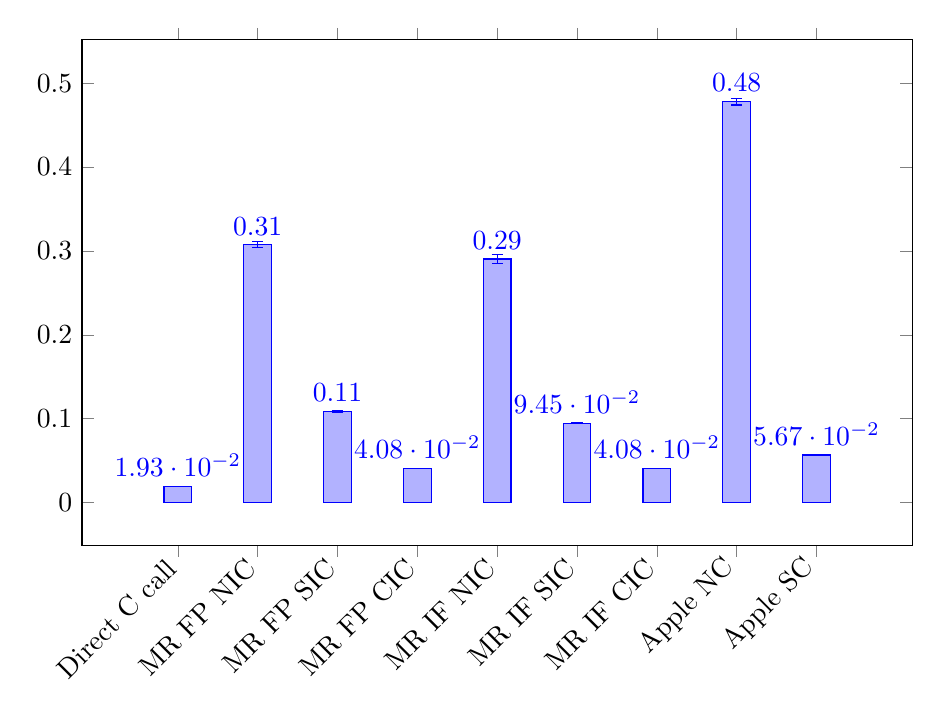
\begin{tikzpicture}
    \begin{axis}[
      ybar,
      width=\textwidth,
      height=8cm,
      enlargelimits=0.15,
      legend style={at={(0.5,-0.2)},
        anchor=north, legend columns=-1},
      symbolic x coords={Direct C call, MR FP NIC, MR FP SIC, MR FP CIC, MR IF NIC, MR IF SIC, MR IF CIC, Apple NC, Apple SC},
      xtick=data, nodes near coords, nodes near coords align={vertical},
      x tick label style={rotate=45,anchor=east},
      ]
      \addplot+[error bars/.cd, y dir=both, y explicit] coordinates {
        (Direct C call, 0.019255) +- (0.002176, 0.000465)
        (MR FP NIC, 0.307301) +- (0.016527, 0.003406)
        (MR FP SIC, 0.108959) +- (0.017548, 0.001271)
        (MR FP CIC, 0.040835) +- (0.000806, 0.000187)
        (MR IF NIC, 0.290375) +- (0.021372, 0.005101)
        (MR IF SIC, 0.094455) +- (0.016948, 0.000674)
        (MR IF CIC, 0.040807) +- (0.001378, 0.000178)
        (Apple NC, 0.478043) +- (0.036600, 0.004128)
        (Apple SC, 0.056732) +- (0.001689, 0.000452)
      };
      
    \end{axis}
  \end{tikzpicture}
  \centering{}
  \caption{Dispatch test - average times.}
  \label{fig:dispatch_test}
\end{figure}

\begin{figure}[H]
  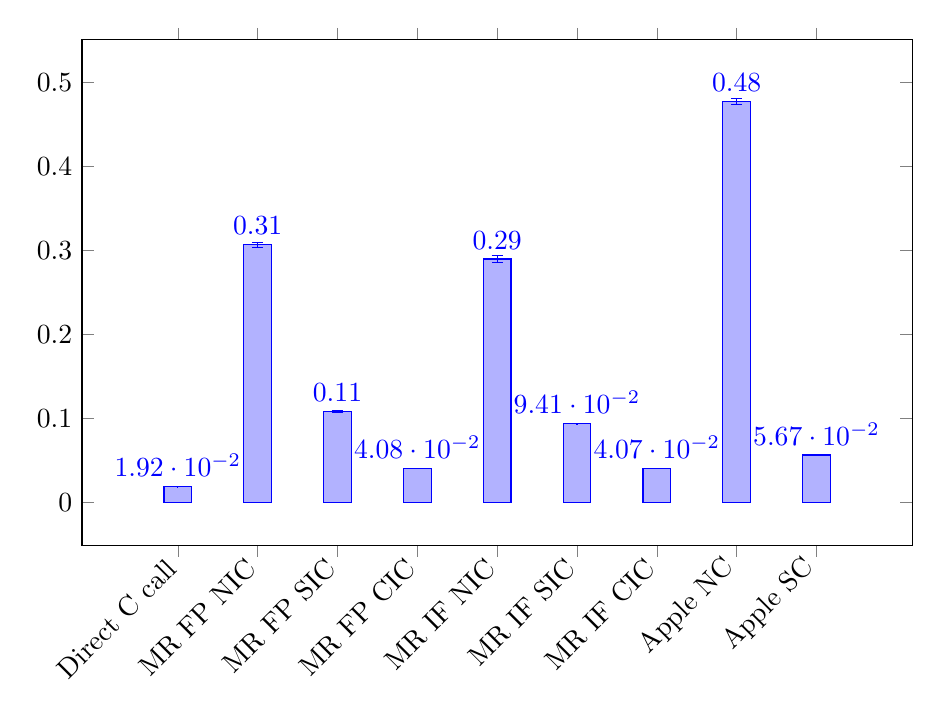
\begin{tikzpicture}
    \begin{axis}[
      ybar,
      width=\textwidth,
      height=8cm,
      enlargelimits=0.15,
      legend style={at={(0.5,-0.2)},
        anchor=north, legend columns=-1},
      symbolic x coords={Direct C call, MR FP NIC, MR FP SIC, MR FP CIC, MR IF NIC, MR IF SIC, MR IF CIC, Apple NC, Apple SC},
      xtick=data, nodes near coords, nodes near coords align={vertical},
      x tick label style={rotate=45,anchor=east},
      ]
      \addplot+[error bars/.cd, y dir=both, y explicit] coordinates {
        (Direct C call, 0.019168) +- (0.002263, 0.000378)
        (MR FP NIC, 0.306875) +- (0.016953, 0.002980)
        (MR FP SIC, 0.108421) +- (0.018086, 0.000733)
        (MR FP CIC, 0.040782) +- (0.000859, 0.000134)
        (MR IF NIC, 0.289886) +- (0.021861, 0.004612)
        (MR IF SIC, 0.094104) +- (0.017299, 0.000323)
        (MR IF CIC, 0.040737) +- (0.001448, 0.000108)
        (Apple NC, 0.477591) +- (0.037052, 0.003676)
        (Apple SC, 0.056659) +- (0.001762, 0.000379)
      };
      
    \end{axis}
  \end{tikzpicture}
  \centering{}
  \caption{Dispatch test - median times.}
  \label{fig:dispatch_test_median}
\end{figure}

\section{Super Dispatch Test}

The method \verb=increment= is added to \verb=MySubclass= as well (overriding the \verb=MyClass=' implementation) and increments the variable \verb=i= as well, while calling \verb=[super increment]=, too. This test is designed to test the speed of calls to \verb=super=.

Results may be seen in figure ~\ref{fig:super_dispatch_test}. Note that the modular run-time does not inline-cache super calls which could probably cut the time in half, beating Apple's run-time, which now beats the modular run-time by 0.03s.

\begin{figure}[H]
  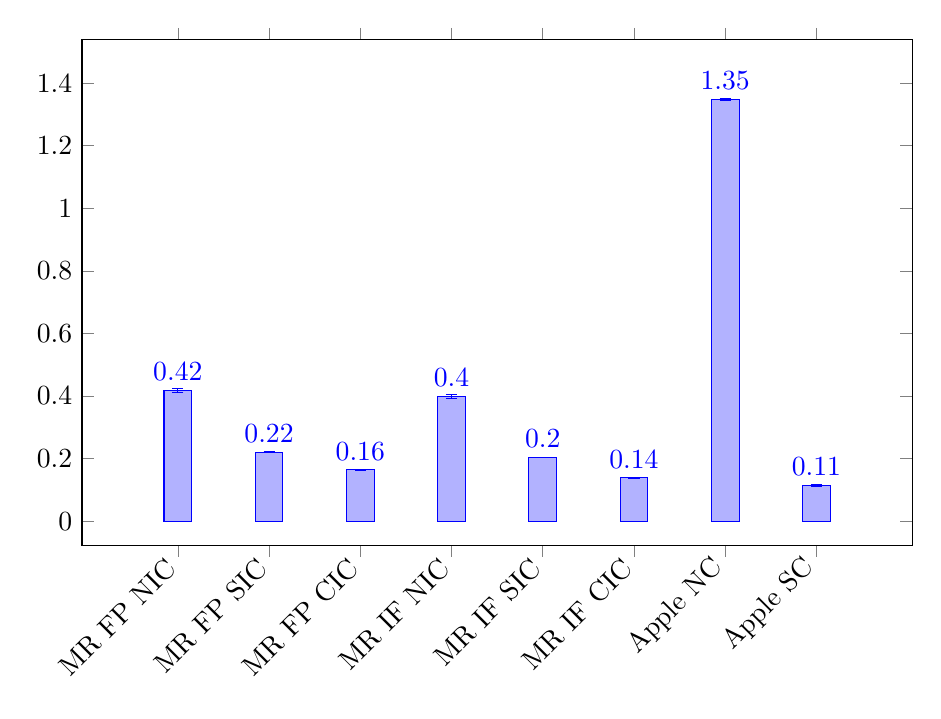
\begin{tikzpicture}
    \begin{axis}[
      ybar,
      width=\textwidth,
      height=8cm,
      enlargelimits=0.15,
      legend style={at={(0.5,-0.2)},
        anchor=north, legend columns=-1},
      symbolic x coords={MR FP NIC, MR FP SIC, MR FP CIC, MR IF NIC, MR IF SIC, MR IF CIC, Apple NC, Apple SC},
      xtick=data, nodes near coords, nodes near coords align={vertical},
      x tick label style={rotate=45,anchor=east},
      ]
      \addplot+[error bars/.cd, y dir=both, y explicit] coordinates {
        (MR FP NIC, 0.417582) +- (0.027834, 0.007497)
        (MR FP SIC, 0.219797) +- (0.017337, 0.001256)
        (MR FP CIC, 0.163980) +- (0.003048, 0.001315)
        (MR IF NIC, 0.399693) +- (0.008895, 0.006510)
        (MR IF SIC, 0.203872) +- (0.008077, 0.000665)
        (MR IF CIC, 0.138670) +- (0.012661, 0.001019)
        (Apple NC, 1.348203) +- (0.070445, 0.004155)
        (Apple SC, 0.113517) +- (0.001528, 0.003764)
      };
      
    \end{axis}
  \end{tikzpicture}
  \centering{}
  \caption{Super dispatch test - average times.}
  \label{fig:super_dispatch_test}
\end{figure}

\begin{figure}[H]
  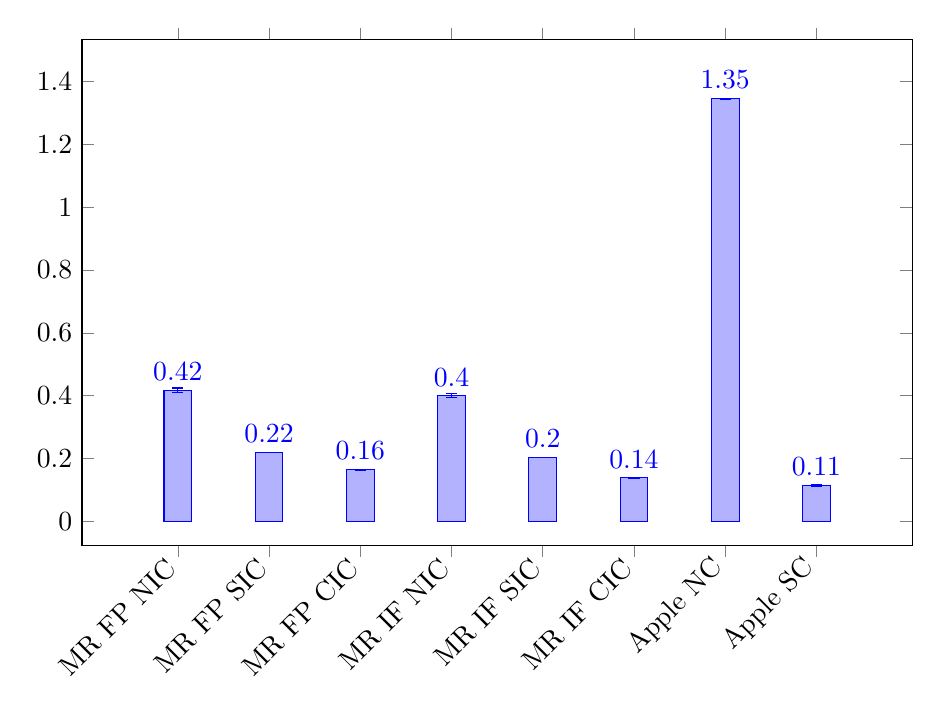
\begin{tikzpicture}
    \begin{axis}[
      ybar,
      width=\textwidth,
      height=8cm,
      enlargelimits=0.15,
      legend style={at={(0.5,-0.2)},
        anchor=north, legend columns=-1},
      symbolic x coords={MR FP NIC, MR FP SIC, MR FP CIC, MR IF NIC, MR IF SIC, MR IF CIC, Apple NC, Apple SC},
      xtick=data, nodes near coords, nodes near coords align={vertical},
      x tick label style={rotate=45,anchor=east},
      ]
      \addplot+[error bars/.cd, y dir=both, y explicit] coordinates {
        (MR FP NIC, 0.417235) +- (0.028181, 0.007150)
        (MR FP SIC, 0.219100) +- (0.018034, 0.000559)
        (MR FP CIC, 0.164129) +- (0.002899, 0.001464)
        (MR IF NIC, 0.399442) +- (0.009146, 0.006259)
        (MR IF SIC, 0.203633) +- (0.008316, 0.000426)
        (MR IF CIC, 0.138173) +- (0.013158, 0.000522)
        (Apple NC, 1.345854) +- (0.072794, 0.001806)
        (Apple SC, 0.113601) +- (0.001444, 0.003848)
      };
      
    \end{axis}
  \end{tikzpicture}
  \centering{}
  \caption{Super dispatch test - median times.}
  \label{fig:super_dispatch_test_median}
\end{figure}

\section{Categories Dispatch Test}

A new method called \verb=incrementViaCategoryMethod=, incrementing the \verb=i= variable in the same way as \verb=increment=, is added to \verb=MyClass= via a class category, which in the modular run-time is implemented as a class extension. This method gets called 10,000,000 times, as in the previous cases.

The results in figure ~\ref{fig:categories_dispatch_test} prove that even class extensions with lookup functions do not slow down the run-time, but even can actually speed up the run-time a little, since the category has only one method, therefore the run-time does not have to go through a method list to fetch the correct method before it caches it for the first time.

\begin{figure}[H]
  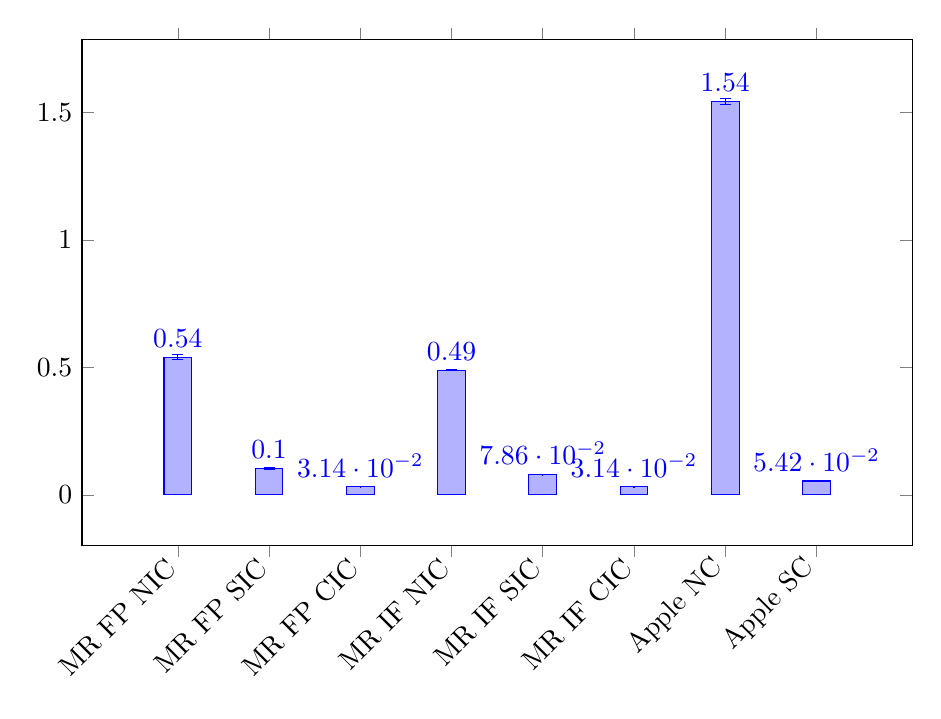
\begin{tikzpicture}
    \begin{axis}[
      ybar,
      width=\textwidth,
      height=8cm,
      enlargelimits=0.15,
      legend style={at={(0.5,-0.2)},
        anchor=north, legend columns=-1},
      symbolic x coords={MR FP NIC, MR FP SIC, MR FP CIC, MR IF NIC, MR IF SIC, MR IF CIC, Apple NC, Apple SC},
      xtick=data, nodes near coords, nodes near coords align={vertical},
      x tick label style={rotate=45,anchor=east},
      ]
      \addplot+[error bars/.cd, y dir=both, y explicit] coordinates {
        (MR FP NIC, 0.540330) +- (0.042624, 0.009375)
        (MR FP SIC, 0.103451) +- (0.014028, 0.002971)
        (MR FP CIC, 0.031401) +- (0.000833, 0.000149)
        (MR IF NIC, 0.488795) +- (0.027994, 0.001599)
        (MR IF SIC, 0.078575) +- (0.012195, 0.000366)
        (MR IF CIC, 0.031366) +- (0.000523, 0.000113)
        (Apple NC, 1.542925) +- (0.054056, 0.013347)
        (Apple SC, 0.054231) +- (0.006432, 0.000543)
      };
      
    \end{axis}
  \end{tikzpicture}
  \centering{}
  \caption{Categories dispatch test - average times.}
  \label{fig:categories_dispatch_test}
\end{figure}

\begin{figure}[H]
  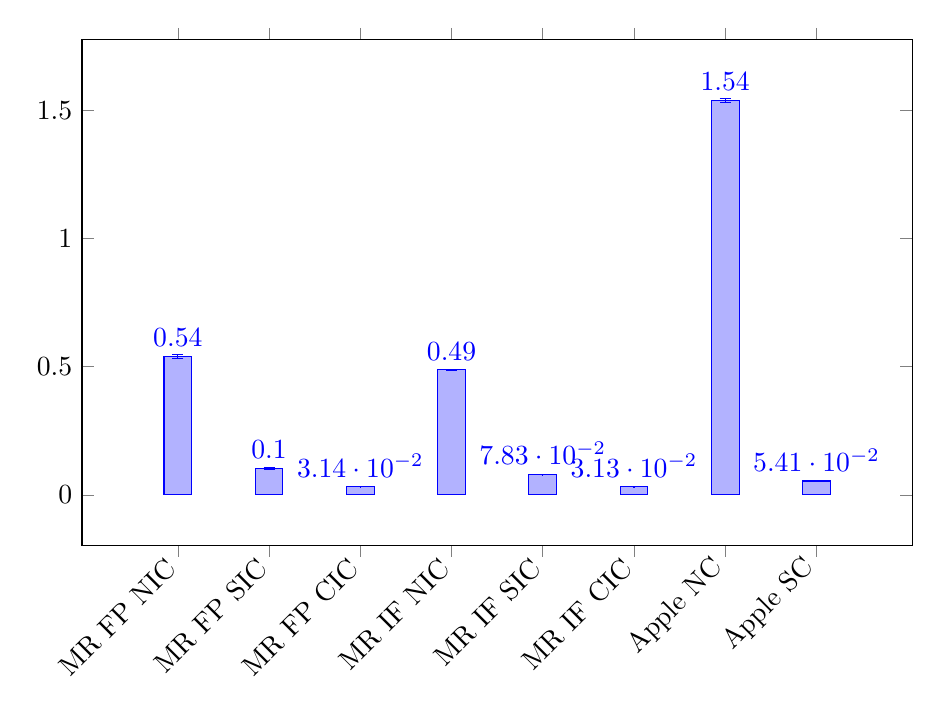
\begin{tikzpicture}
    \begin{axis}[
      ybar,
      width=\textwidth,
      height=8cm,
      enlargelimits=0.15,
      legend style={at={(0.5,-0.2)},
        anchor=north, legend columns=-1},
      symbolic x coords={MR FP NIC, MR FP SIC, MR FP CIC, MR IF NIC, MR IF SIC, MR IF CIC, Apple NC, Apple SC},
      xtick=data, nodes near coords, nodes near coords align={vertical},
      x tick label style={rotate=45,anchor=east},
      ]
      \addplot+[error bars/.cd, y dir=both, y explicit] coordinates {
        (MR FP NIC, 0.539607) +- (0.043347, 0.008652)
        (MR FP SIC, 0.102974) +- (0.014505, 0.002494)
        (MR FP CIC, 0.031357) +- (0.000877, 0.000105)
        (MR IF NIC, 0.487892) +- (0.028897, 0.000696)
        (MR IF SIC, 0.078346) +- (0.012424, 0.000137)
        (MR IF CIC, 0.031341) +- (0.000548, 0.000088)
        (Apple NC, 1.539003) +- (0.057978, 0.009425)
        (Apple SC, 0.054104) +- (0.006559, 0.000416)
      };
      
    \end{axis}
  \end{tikzpicture}
  \centering{}
  \caption{Categories dispatch test - median times.}
  \label{fig:categories_dispatch_test_median}
\end{figure}


\section{Allocation Test}

In a cycle, an instance of \verb=MyClass= is allocated and immediately deallocated for 10,000,000 times.

Since this test does not use the dispatch, inline caching has no effect on the results as can be seen on figure ~\ref{fig:alloc_test}. You can see, however, the benefit of function inlining here, which completes the allocation test 0.01s faster than using function pointers.

\begin{figure}[H]
  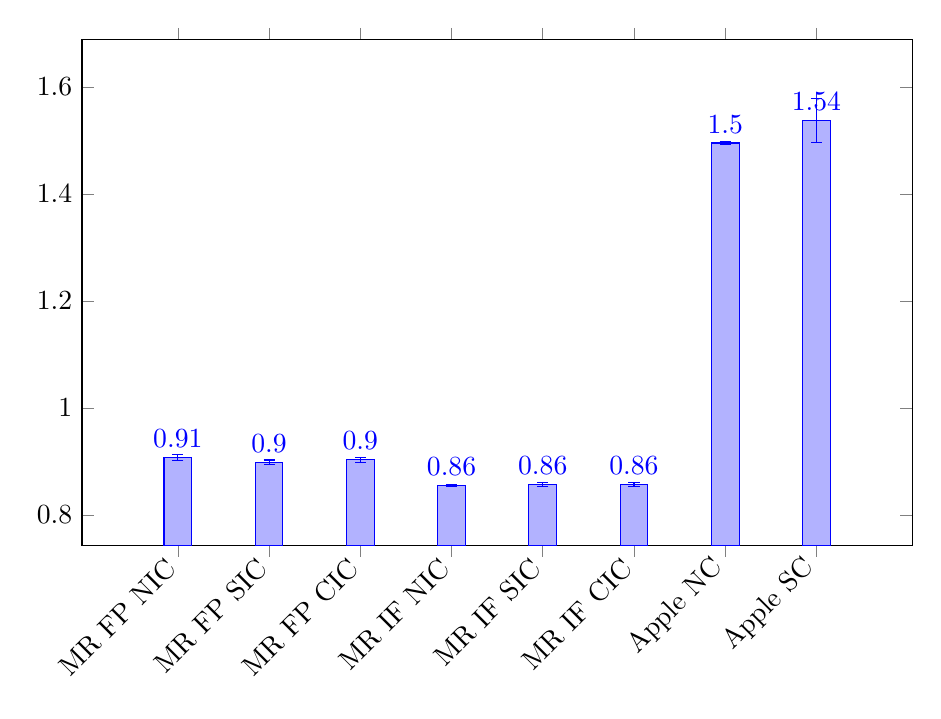
\begin{tikzpicture}
    \begin{axis}[
      ybar,
      width=\textwidth,
      height=8cm,
      enlargelimits=0.15,
      legend style={at={(0.5,-0.2)},
        anchor=north, legend columns=-1},
      symbolic x coords={MR FP NIC, MR FP SIC, MR FP CIC, MR IF NIC, MR IF SIC, MR IF CIC, Apple NC, Apple SC},
      xtick=data, nodes near coords, nodes near coords align={vertical},
      x tick label style={rotate=45,anchor=east},
      ]
      \addplot+[error bars/.cd, y dir=both, y explicit] coordinates {
        (MR FP NIC, 0.907829) +- (0.029326, 0.005914)
        (MR FP SIC, 0.898413) +- (0.008233, 0.004408)
        (MR FP CIC, 0.903404) +- (0.055865, 0.004459)
        (MR IF NIC, 0.855232) +- (0.013685, 0.001611)
        (MR IF SIC, 0.856829) +- (0.069212, 0.003546)
        (MR IF CIC, 0.856930) +- (0.021839, 0.004196)
        (Apple NC, 1.495227) +- (0.017146, 0.001874)
        (Apple SC, 1.537473) +- (0.305385, 0.041753)
      };
      
    \end{axis}
  \end{tikzpicture}
  \centering{}
  \caption{Allocation test - average times.}
  \label{fig:alloc_test}
\end{figure}

\begin{figure}[H]
  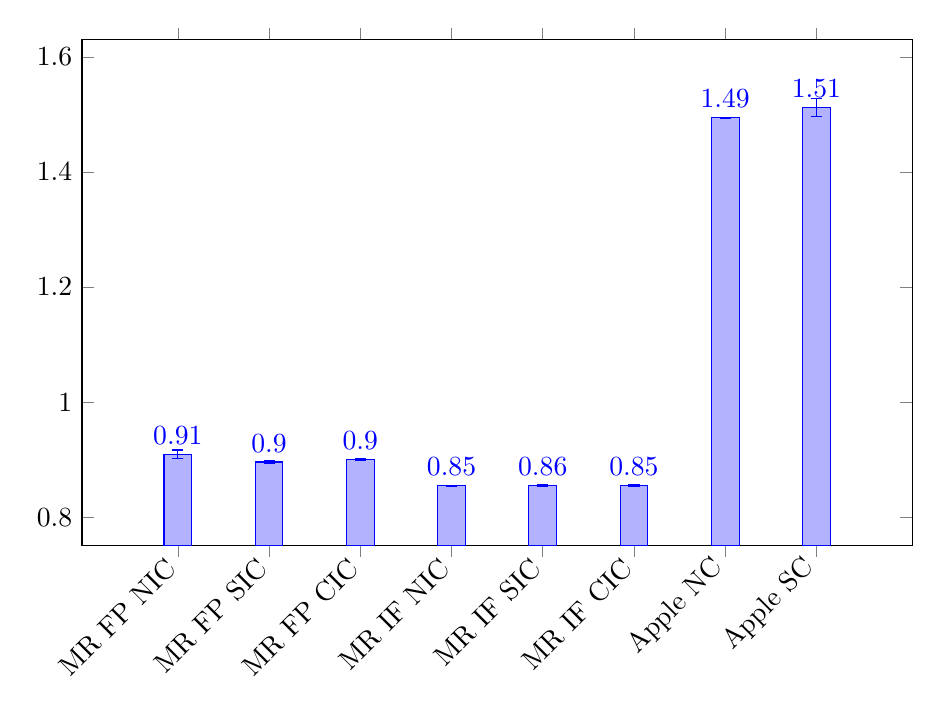
\begin{tikzpicture}
    \begin{axis}[
      ybar,
      width=\textwidth,
      height=8cm,
      enlargelimits=0.15,
      legend style={at={(0.5,-0.2)},
        anchor=north, legend columns=-1},
      symbolic x coords={MR FP NIC, MR FP SIC, MR FP CIC, MR IF NIC, MR IF SIC, MR IF CIC, Apple NC, Apple SC},
      xtick=data, nodes near coords, nodes near coords align={vertical},
      x tick label style={rotate=45,anchor=east},
      ]
      \addplot+[error bars/.cd, y dir=both, y explicit] coordinates {
        (MR FP NIC, 0.909304) +- (0.027851, 0.007389)
        (MR FP SIC, 0.895909) +- (0.010737, 0.001904)
        (MR FP CIC, 0.900434) +- (0.058835, 0.001489)
        (MR IF NIC, 0.854637) +- (0.014280, 0.001016)
        (MR IF SIC, 0.855065) +- (0.070976, 0.001782)
        (MR IF CIC, 0.854746) +- (0.024023, 0.002012)
        (Apple NC, 1.494171) +- (0.018202, 0.000818)
        (Apple SC, 1.512026) +- (0.330832, 0.016306)
      };
      
    \end{axis}
  \end{tikzpicture}
  \centering{}
  \caption{Allocation test - median times.}
  \label{fig:alloc_test_median}
\end{figure}


\section{Ivar Test}

An instance of \verb=MySubclass= is created and 10,000,000 times, its method \newline{}\verb=incrementViaSettersAndGetters= is called. This method does not directly access the \verb=i= ivar, but rather uses run-time functions to modify it.

This test interlaces the dispatch test with calling run-time functions, which, as can be seen on figure ~\ref{fig:ivar_test}, again proves that Apple's run-time is incredibly slow at fetching selectors and at using the ivar fetching functions. Note that as it is fetching ivars, which cannot be added after the class has been registered with the run-time, no locks should be necessary.

\begin{figure}[H]
  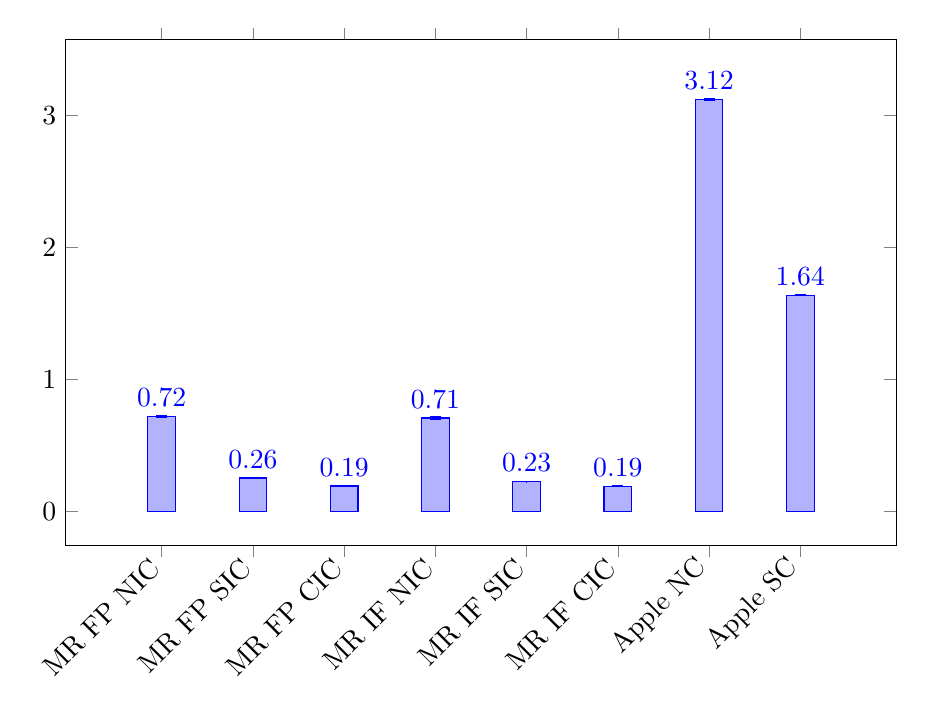
\begin{tikzpicture}
    \begin{axis}[
      ybar,
      width=\textwidth,
      height=8cm,
      enlargelimits=0.15,
      legend style={at={(0.5,-0.2)},
        anchor=north, legend columns=-1},
      symbolic x coords={MR FP NIC, MR FP SIC, MR FP CIC, MR IF NIC, MR IF SIC, MR IF CIC, Apple NC, Apple SC},
      xtick=data, nodes near coords, nodes near coords align={vertical},
      x tick label style={rotate=45,anchor=east},
      ]
      \addplot+[error bars/.cd, y dir=both, y explicit] coordinates {
        (MR FP NIC, 0.720783) +- (0.040378, 0.007518)
        (MR FP SIC, 0.255136) +- (0.043586, 0.002016)
        (MR FP CIC, 0.194685) +- (0.021604, 0.001956)
        (MR IF NIC, 0.709346) +- (0.029565, 0.012094)
        (MR IF SIC, 0.228298) +- (0.051006, 0.002174)
        (MR IF CIC, 0.191331) +- (0.015678, 0.003138)
        (Apple NC, 3.123157) +- (0.100556, 0.008450)
        (Apple SC, 1.639187) +- (0.032947, 0.004935)
      };
      
    \end{axis}
  \end{tikzpicture}
  \centering{}
  \caption{Ivar test - average times.}
  \label{fig:ivar_test}
\end{figure}

\begin{figure}[H]
  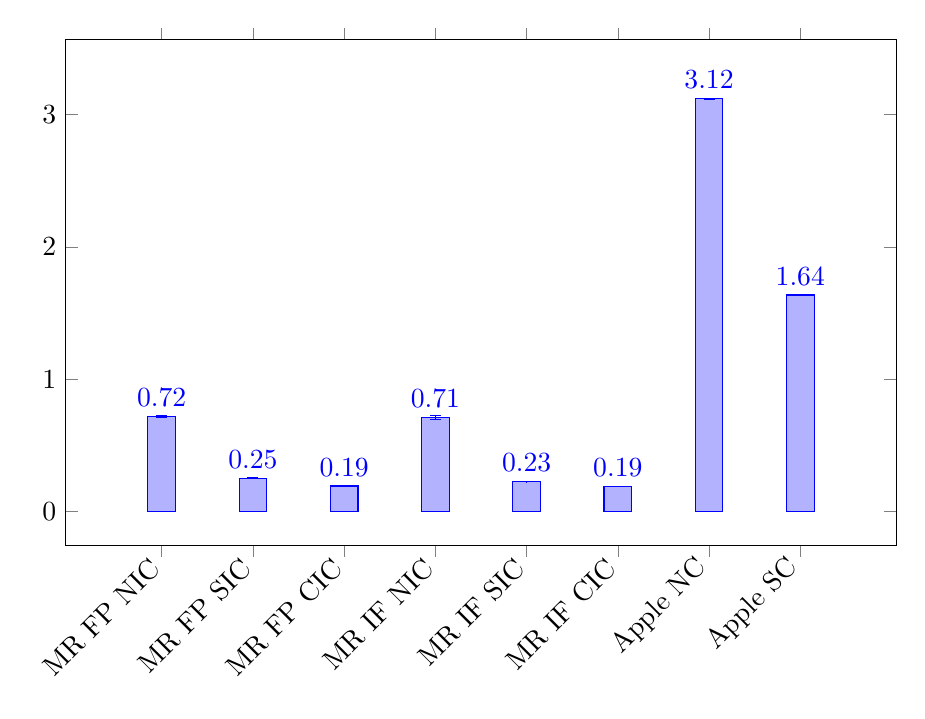
\begin{tikzpicture}
    \begin{axis}[
      ybar,
      width=\textwidth,
      height=8cm,
      enlargelimits=0.15,
      legend style={at={(0.5,-0.2)},
        anchor=north, legend columns=-1},
      symbolic x coords={MR FP NIC, MR FP SIC, MR FP CIC, MR IF NIC, MR IF SIC, MR IF CIC, Apple NC, Apple SC},
      xtick=data, nodes near coords, nodes near coords align={vertical},
      x tick label style={rotate=45,anchor=east},
      ]
      \addplot+[error bars/.cd, y dir=both, y explicit] coordinates {
        (MR FP NIC, 0.718906) +- (0.042255, 0.005641)
        (MR FP SIC, 0.254027) +- (0.044695, 0.000907)
        (MR FP CIC, 0.194400) +- (0.021889, 0.001671)
        (MR IF NIC, 0.710597) +- (0.028314, 0.013345)
        (MR IF SIC, 0.226814) +- (0.052490, 0.000690)
        (MR IF CIC, 0.191008) +- (0.016001, 0.002815)
        (Apple NC, 3.118531) +- (0.105182, 0.003824)
        (Apple SC, 1.636454) +- (0.035680, 0.002202)
      };
      
    \end{axis}
  \end{tikzpicture}
  \centering{}
  \caption{Ivar test - median times.}
  \label{fig:ivar_test_median}
\end{figure}


\section{Forwarding Test}

A third class \verb=NewClass= is created with a single method \verb=unknownSelector:=. An instance of \verb=MySubclass= is created and the \verb=proxyObject= ivar is set to an instance of \verb=NewClass=. \verb=MyClass= implements the run-time's forwarding mechanism and all unknown calls are directed to the \verb=proxyObject=. This test compares the direct calls to the \verb=NewClass= instance with proxy calls.

As has been noted above, Apple has two forwarding mechanisms, one obsolete, using the \verb=forward::= method, the other introduced by the Foundation framework and generally the only one that should be used, since the \verb=objc_msgSendv=, which would accept the arguments list, is deprecated with no alternative. This test, nevertheless, is also testing this deprecated method, in tests marked as \verb=Apple NC 2= and \verb=Apple SC 2=. As can be seen, figure ~\ref{fig:forwarding_test}, wrapping the calls in \verb=NSInvocation= objects is very costly and makes the calls extremely slow. Note that the inner cycle body needed to be wrapped in an \verb=@autorelease= block to prevent excess memory usage.

The complete inline caching versions of the test achieve nearly the speed of the regular dispatch test, since the \verb=objc_object_lookup_method= function returns directly the forwarded method.

\begin{figure}[H]
  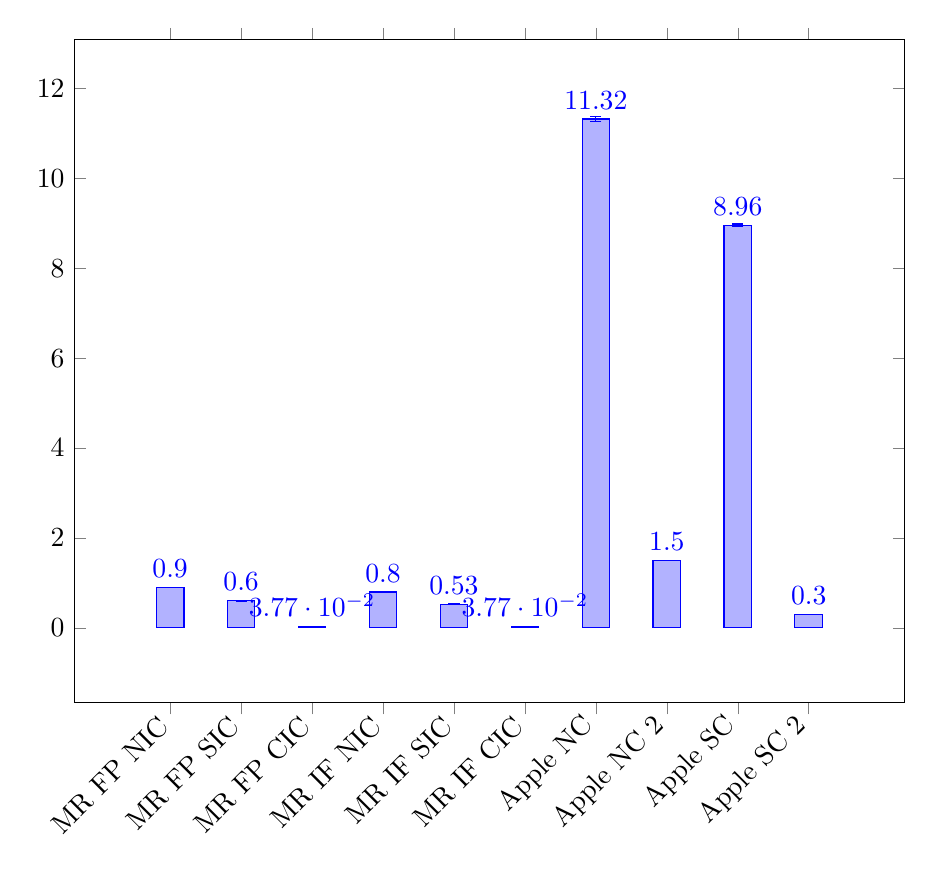
\begin{tikzpicture}
    \begin{axis}[
      ybar,
      width=\textwidth,
      height=10cm,
      enlargelimits=0.15,
      legend style={at={(0.5,-0.2)},
        anchor=south, legend columns=-1},
      symbolic x coords={MR FP NIC, MR FP SIC, MR FP CIC, MR IF NIC, MR IF SIC, MR IF CIC, Apple NC, Apple NC 2, Apple SC, Apple SC 2},
      xtick=data, nodes near coords, nodes near coords align={vertical},
      x tick label style={rotate=45,anchor=east},
      ]
      \addplot+[error bars/.cd, y dir=both, y explicit] coordinates {
        (MR FP NIC, 0.897772) +- (0.057546, 0.007078)
        (MR FP SIC, 0.602062) +- (0.049864, 0.009191)
        (MR FP CIC, 0.037677) +- (0.000449, 0.000174)
        (MR IF NIC, 0.797122) +- (0.041635, 0.007196)
        (MR IF SIC, 0.527963) +- (0.029939, 0.001566)
        (MR IF CIC, 0.037669) +- (0.000533, 0.000166)
        (Apple NC, 11.321042) +- (0.412569, 0.060302)
        (Apple NC 2, 1.498870) +- (0.067623, 0.004295)
        (Apple SC, 8.958324) +- (0.108468, 0.026535)
        (Apple SC 2, 0.297697) +- (0.008523, 0.001189)
      };
      
    \end{axis}
  \end{tikzpicture}
  \centering{}
  \caption{Forwarding test - average times.}
  \label{fig:forwarding_test}
\end{figure}

\begin{figure}[H]
  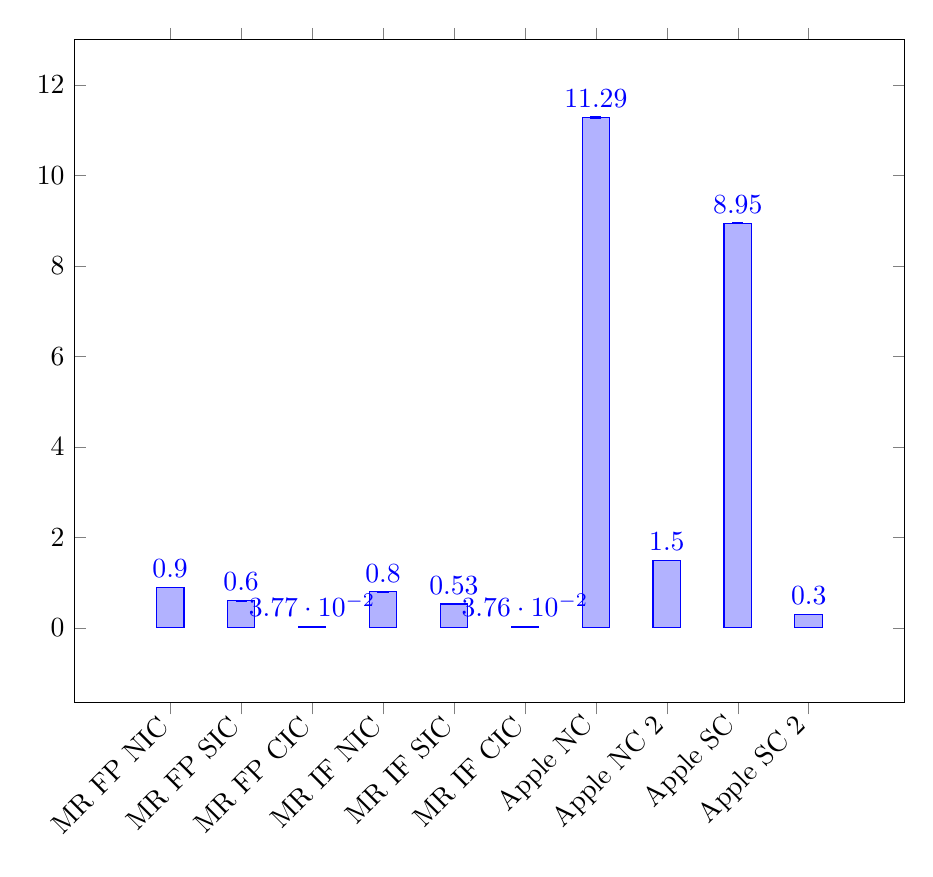
\begin{tikzpicture}
    \begin{axis}[
      ybar,
      width=\textwidth,
      height=10cm,
      enlargelimits=0.15,
      legend style={at={(0.5,-0.2)},
        anchor=south, legend columns=-1},
      symbolic x coords={MR FP NIC, MR FP SIC, MR FP CIC, MR IF NIC, MR IF SIC, MR IF CIC, Apple NC, Apple NC 2, Apple SC, Apple SC 2},
      xtick=data, nodes near coords, nodes near coords align={vertical},
      x tick label style={rotate=45,anchor=east},
      ]
      \addplot+[error bars/.cd, y dir=both, y explicit] coordinates {
        (MR FP NIC, 0.895417) +- (0.059901, 0.004723)
        (MR FP SIC, 0.601379) +- (0.050547, 0.008508)
        (MR FP CIC, 0.037652) +- (0.000474, 0.000149)
        (MR IF NIC, 0.797237) +- (0.041520, 0.007311)
        (MR IF SIC, 0.526907) +- (0.030995, 0.000510)
        (MR IF CIC, 0.037649) +- (0.000553, 0.000146)
        (Apple NC, 11.285208) +- (0.448403, 0.024468)
        (Apple NC 2, 1.496482) +- (0.070011, 0.001907)
        (Apple SC, 8.946234) +- (0.120558, 0.014445)
        (Apple SC 2, 0.297470) +- (0.008750, 0.000962)
      };
      
    \end{axis}
  \end{tikzpicture}
  \centering{}
  \caption{Forwarding test - median times.}
  \label{fig:forwarding_test_median}
\end{figure}

\section{Associated Objects Test}

This test uses associated objects, to store an integer value (\verb=i=) and increment it 10,000,000 times.

Figure ~\ref{fig:ao_test} proves the suspicion that Apple's implementation of associated objects has a bottle neck in the spin lock and external structure.

\begin{figure}[H]
  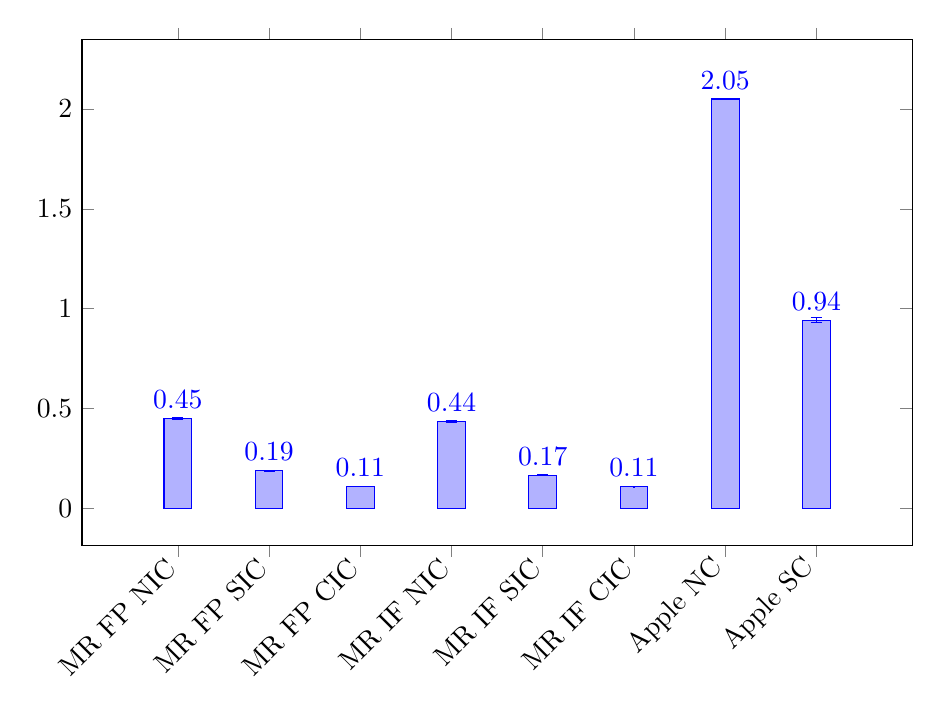
\begin{tikzpicture}
    \begin{axis}[
      ybar,
      width=\textwidth,
      height=8cm,
      enlargelimits=0.15,
      legend style={at={(0.5,-0.2)},
        anchor=north, legend columns=-1, /pgf/number format/.cd precision=3},
      symbolic x coords={MR FP NIC, MR FP SIC, MR FP CIC, MR IF NIC, MR IF SIC, MR IF CIC, Apple NC, Apple SC},
      xtick=data, nodes near coords, nodes near coords align={vertical},
      x tick label style={rotate=45,anchor=east},
      ]
      \addplot+[error bars/.cd, y dir=both, y explicit] coordinates {
        (MR FP NIC, 0.449866) +- (0.027097, 0.003849)
        (MR FP SIC, 0.187626) +- (0.022911, 0.003433)
        (MR FP CIC, 0.108897) +- (0.023050, 0.001543)
        (MR IF NIC, 0.436402) +- (0.031055, 0.004886)
        (MR IF SIC, 0.165698) +- (0.019138, 0.001920)
        (MR IF CIC, 0.108241) +- (0.023137, 0.001155)
        (Apple NC, 2.050271) +- (0.088587, 0.004679)
        (Apple SC, 0.941849) +- (0.110477, 0.013326)
      };
      
    \end{axis}
  \end{tikzpicture}
  \centering{}
  \caption{Associated objects test - average times.}
  \label{fig:ao_test}
\end{figure}

\begin{figure}[H]
  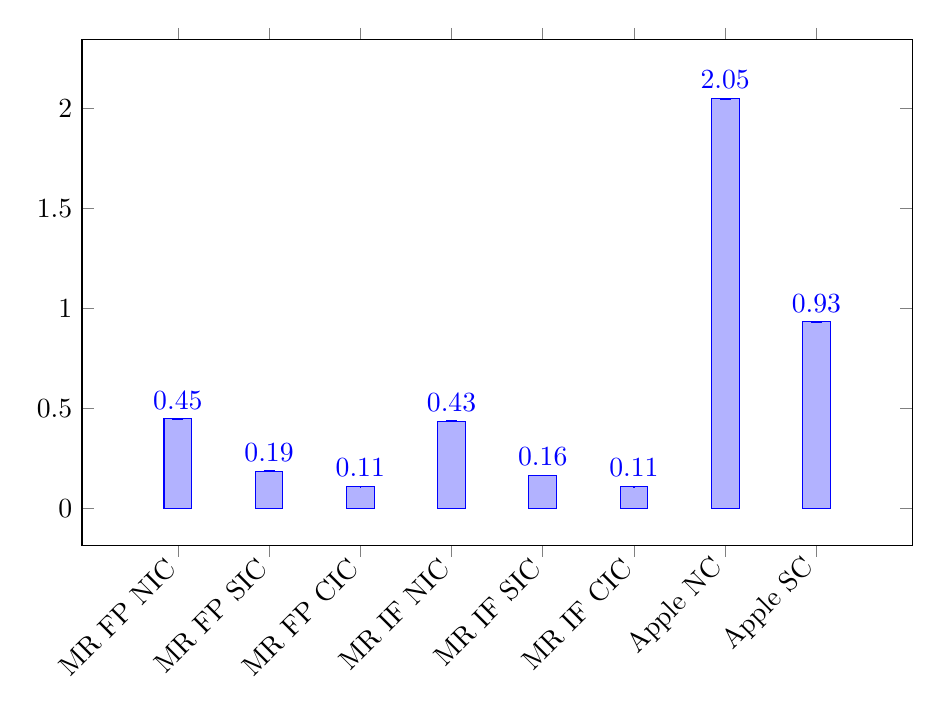
\begin{tikzpicture}
    \begin{axis}[
      ybar,
      width=\textwidth,
      height=8cm,
      enlargelimits=0.15,
      legend style={at={(0.5,-0.2)},
        anchor=north, legend columns=-1, /pgf/number format/.cd precision=3},
      symbolic x coords={MR FP NIC, MR FP SIC, MR FP CIC, MR IF NIC, MR IF SIC, MR IF CIC, Apple NC, Apple SC},
      xtick=data, nodes near coords, nodes near coords align={vertical},
      x tick label style={rotate=45,anchor=east},
      ]
      \addplot+[error bars/.cd, y dir=both, y explicit] coordinates {
        (MR FP NIC, 0.446899) +- (0.030064, 0.000882)
        (MR FP SIC, 0.185234) +- (0.025303, 0.001041)
        (MR FP CIC, 0.107822) +- (0.024125, 0.000468)
        (MR IF NIC, 0.434640) +- (0.032817, 0.003124)
        (MR IF SIC, 0.164623) +- (0.020213, 0.000845)
        (MR IF CIC, 0.107422) +- (0.023956, 0.000336)
        (Apple NC, 2.047889) +- (0.090969, 0.002297)
        (Apple SC, 0.931327) +- (0.120999, 0.002804)
      };
      
    \end{axis}
  \end{tikzpicture}
  \centering{}
  \caption{Associated objects test - median times.}
  \label{fig:ao_test_median}
\end{figure}


